\documentclass{standalone}
\usepackage{tikz}
\usetikzlibrary{patterns, positioning}
\usetikzlibrary{shapes.misc}
\usepackage[outline]{contour}
\contourlength{1.5pt} 
\usepackage[sfdefault]{ClearSans} %% option 'sfdefault' activates Clear Sans as the default text font
\usepackage[T1]{fontenc}

\begin{document}
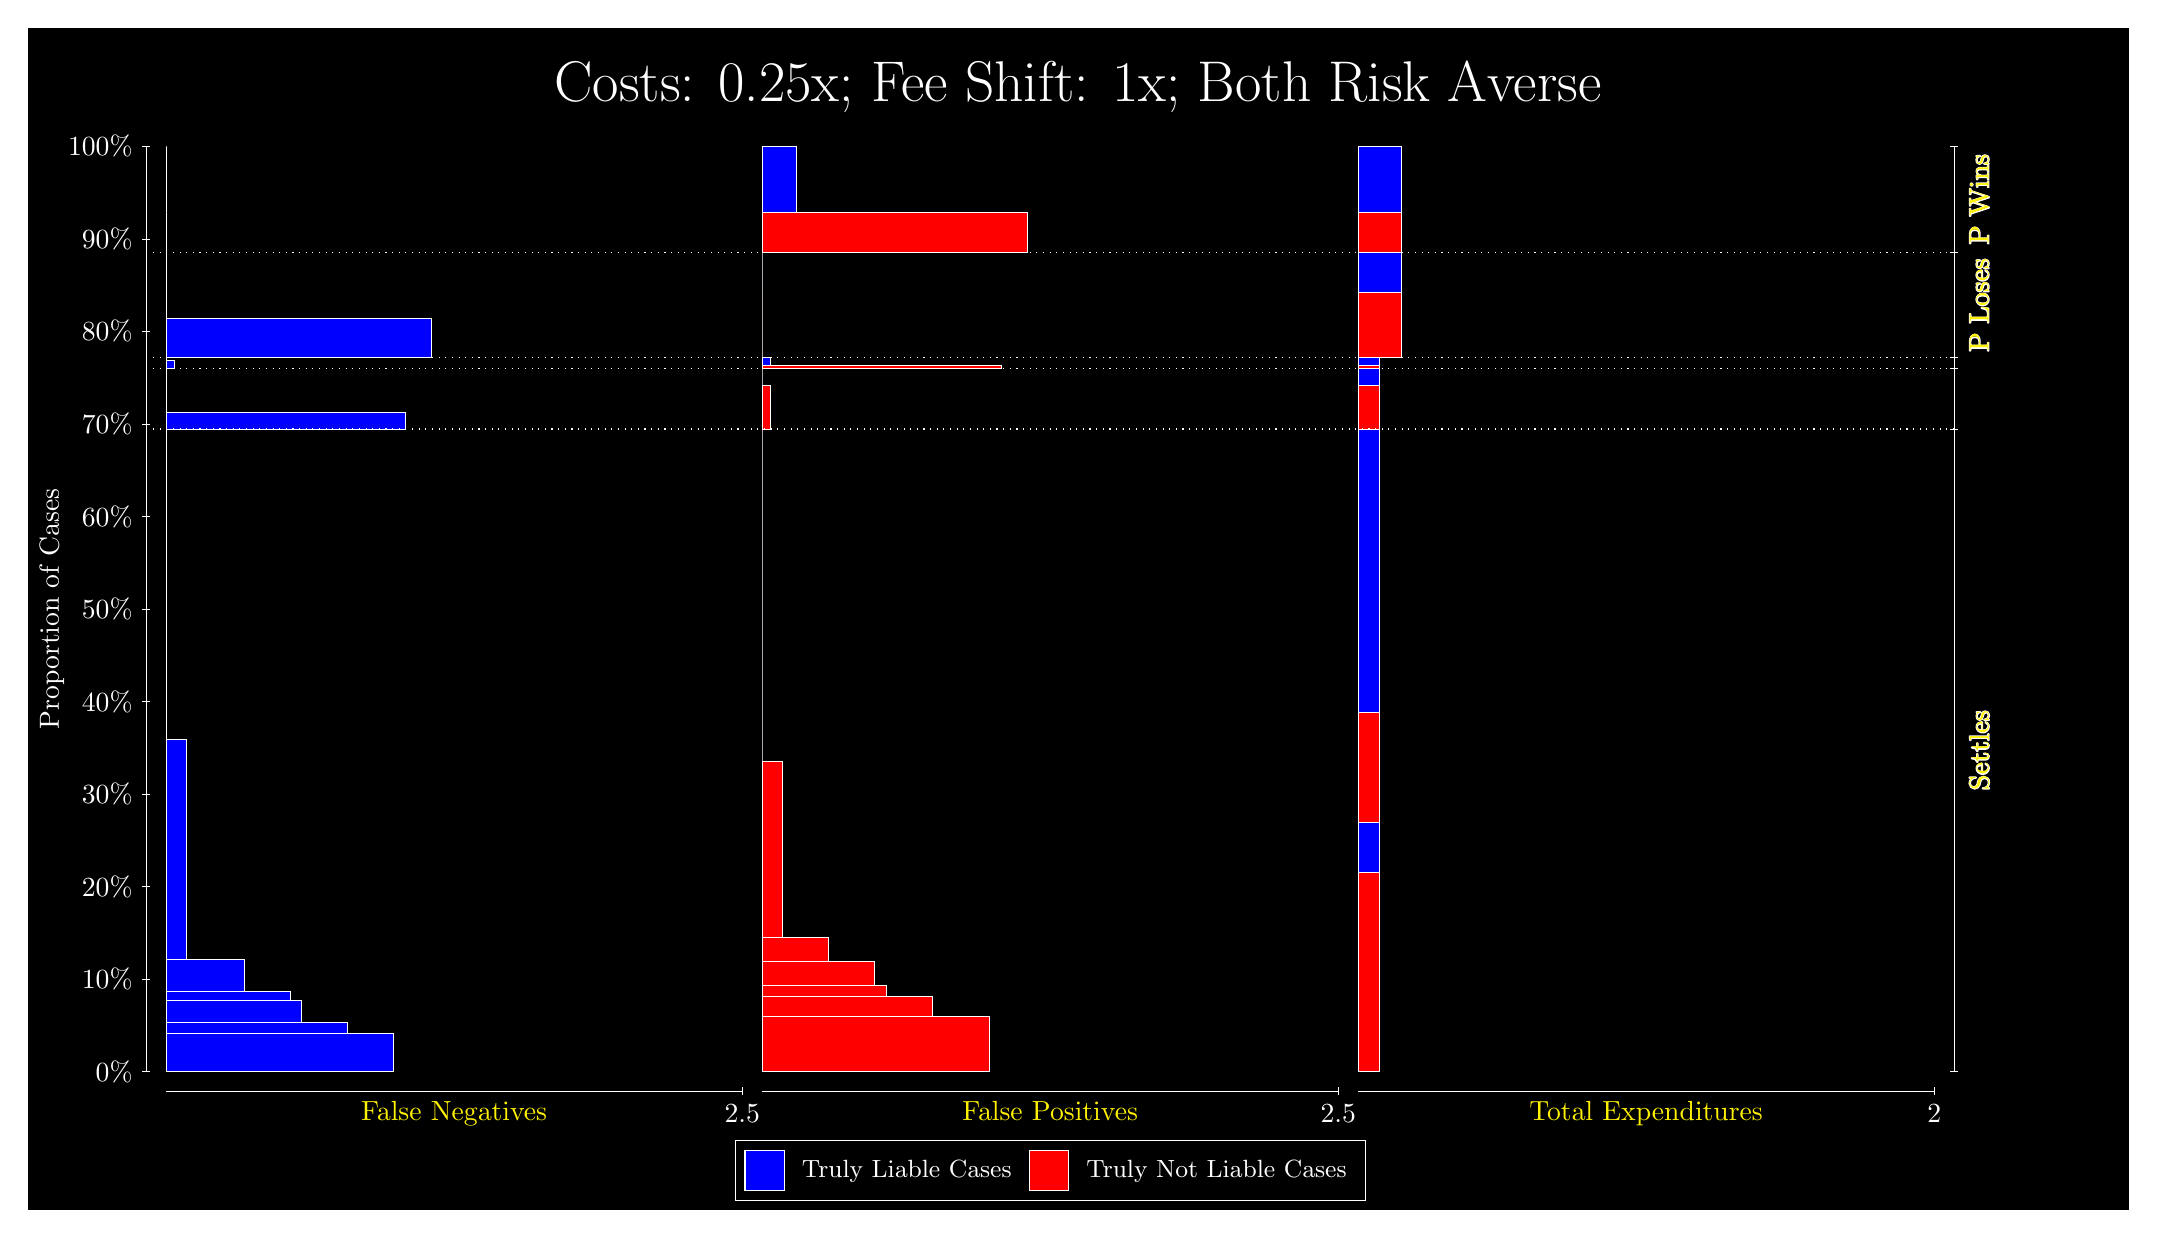
\begin{tikzpicture}
\draw[fill=black] (0,0) rectangle (26.667,15);
\draw[text=white] (0,13.5) rectangle (26.667,15) node[midway] {\huge Costs: 0.25x; Fee Shift: 1x; Both Risk Averse};
\draw[white, very thin] (1.5,1.75) -- (1.5,13.5);
\node[rotate=90, text=white, anchor=center] at (0.3, 7.625) {Proportion of Cases};
\draw[white, very thin] (1.45,1.75) -- (1.55,1.75);
\node[text=white, anchor=east] at (1.45, 1.75) {0\%};
\draw[white, very thin] (1.45,2.925) -- (1.55,2.925);
\node[text=white, anchor=east] at (1.45, 2.925) {10\%};
\draw[white, very thin] (1.45,4.1) -- (1.55,4.1);
\node[text=white, anchor=east] at (1.45, 4.1) {20\%};
\draw[white, very thin] (1.45,5.275) -- (1.55,5.275);
\node[text=white, anchor=east] at (1.45, 5.275) {30\%};
\draw[white, very thin] (1.45,6.45) -- (1.55,6.45);
\node[text=white, anchor=east] at (1.45, 6.45) {40\%};
\draw[white, very thin] (1.45,7.625) -- (1.55,7.625);
\node[text=white, anchor=east] at (1.45, 7.625) {50\%};
\draw[white, very thin] (1.45,8.8) -- (1.55,8.8);
\node[text=white, anchor=east] at (1.45, 8.8) {60\%};
\draw[white, very thin] (1.45,9.975) -- (1.55,9.975);
\node[text=white, anchor=east] at (1.45, 9.975) {70\%};
\draw[white, very thin] (1.45,11.15) -- (1.55,11.15);
\node[text=white, anchor=east] at (1.45, 11.15) {80\%};
\draw[white, very thin] (1.45,12.325) -- (1.55,12.325);
\node[text=white, anchor=east] at (1.45, 12.325) {90\%};
\draw[white, very thin] (1.45,13.5) -- (1.55,13.5);
\node[text=white, anchor=east] at (1.45, 13.5) {100\%};

\draw[white, very thin] (24.457,1.75) -- (24.457,13.5);
\draw[white, very thin] (24.407,1.75) -- (24.507,1.75);
\node[anchor=west] at (24.407, 1.75) {};
\draw[white, very thin] (24.407,9.91) -- (24.507,9.91);
\node[anchor=west] at (24.407, 9.91) {};
\draw[white, very thin] (24.407,10.678) -- (24.507,10.678);
\node[anchor=west] at (24.407, 10.678) {};
\draw[white, very thin] (24.407,10.815) -- (24.507,10.815);
\node[anchor=west] at (24.407, 10.815) {};
\draw[white, very thin] (24.407,12.153) -- (24.507,12.153);
\node[anchor=west] at (24.407, 12.153) {};
\draw[white, very thin] (24.407,13.5) -- (24.507,13.5);
\node[anchor=west] at (24.407, 13.5) {};

\draw[white, very thin, fill=blue] (1.75,1.75) rectangle (4.641,2.2346);
\draw[white, very thin, fill=blue] (1.75,2.2346) rectangle (4.0554,2.3781);
\draw[white, very thin, fill=blue] (1.75,2.3781) rectangle (3.4699,2.656);
\draw[white, very thin, fill=blue] (1.75,2.656) rectangle (3.3236,2.7634);
\draw[white, very thin, fill=blue] (1.75,2.7634) rectangle (2.738,3.1807);
\draw[white, very thin, fill=blue] (1.75,3.1807) rectangle (2.0062,5.9725);
\draw[white, very thin, fill=red] (1.75,5.9725) rectangle (1.75,9.91);
\draw[white, very thin, fill=blue] (1.75,9.91) rectangle (4.7873,10.118);
\draw[white, very thin, fill=red] (1.75,10.118) rectangle (1.75,10.678);
\draw[white, very thin, fill=blue] (1.75,10.678) rectangle (1.8598,10.777);
\draw[white, very thin, fill=red] (1.75,10.777) rectangle (1.75,10.815);
\draw[white, very thin, fill=blue] (1.75,10.815) rectangle (5.1167,11.321);
\draw[white, very thin, fill=red] (1.75,11.321) rectangle (1.75,12.153);
\draw[white, very thin, fill=red] (1.75,12.153) rectangle (1.75,12.661);
\draw[white, very thin, fill=blue] (1.75,12.661) rectangle (1.75,13.5);
\draw[white, very thin, fill=red] (9.3189,1.75) rectangle (12.21,2.4508);
\draw[white, very thin, fill=red] (9.3189,2.4508) rectangle (11.478,2.7117);
\draw[white, very thin, fill=red] (9.3189,2.7117) rectangle (10.892,2.8393);
\draw[white, very thin, fill=red] (9.3189,2.8393) rectangle (10.746,3.1551);
\draw[white, very thin, fill=red] (9.3189,3.1551) rectangle (10.161,3.4569);
\draw[white, very thin, fill=red] (9.3189,3.4569) rectangle (9.575,5.6875);
\draw[white, very thin, fill=blue] (9.3189,5.6875) rectangle (9.3189,9.91);
\draw[white, very thin, fill=red] (9.3189,9.91) rectangle (9.4287,10.47);
\draw[white, very thin, fill=blue] (9.3189,10.47) rectangle (9.3189,10.678);
\draw[white, very thin, fill=red] (9.3189,10.678) rectangle (12.356,10.716);
\draw[white, very thin, fill=blue] (9.3189,10.716) rectangle (9.4287,10.815);
\draw[white, very thin, fill=red] (9.3189,10.815) rectangle (9.3189,11.647);
\draw[white, very thin, fill=blue] (9.3189,11.647) rectangle (9.3189,12.153);
\draw[white, very thin, fill=red] (9.3189,12.153) rectangle (12.686,12.661);
\draw[white, very thin, fill=blue] (9.3189,12.661) rectangle (9.758,13.5);
\draw[white, very thin, fill=red] (16.888,1.75) rectangle (17.162,4.2824);
\draw[white, very thin, fill=blue] (16.888,4.2824) rectangle (17.162,4.9106);
\draw[white, very thin, fill=red] (16.888,4.9106) rectangle (17.162,6.3156);
\draw[white, very thin, fill=blue] (16.888,6.3156) rectangle (17.162,9.91);
\draw[white, very thin, fill=red] (16.888,9.91) rectangle (17.162,10.47);
\draw[white, very thin, fill=blue] (16.888,10.47) rectangle (17.162,10.678);
\draw[white, very thin, fill=red] (16.888,10.678) rectangle (17.162,10.716);
\draw[white, very thin, fill=blue] (16.888,10.716) rectangle (17.162,10.815);
\draw[white, very thin, fill=red] (16.888,10.815) rectangle (17.437,11.647);
\draw[white, very thin, fill=blue] (16.888,11.647) rectangle (17.437,12.153);
\draw[white, very thin, fill=red] (16.888,12.153) rectangle (17.437,12.661);
\draw[white, very thin, fill=blue] (16.888,12.661) rectangle (17.437,13.5);
\draw[white, dotted] (1.5,9.91) -- (24.457,9.91);
\draw[white, dotted] (1.5,10.678) -- (24.457,10.678);
\draw[white, dotted] (1.5,10.815) -- (24.457,10.815);
\draw[white, dotted] (1.5,12.153) -- (24.457,12.153);
\draw[white, very thin] (1.75,1.5) -- (9.0689,1.5);
\node[text=yellow, anchor=north] at (5.4094, 1.5) {False Negatives};
\draw[white, very thin] (9.0689,1.45) -- (9.0689,1.55);
\node[text=white, anchor=north] at (9.0689, 1.45) {2.5};

\draw[white, very thin] (9.3189,1.5) -- (16.638,1.5);
\node[text=yellow, anchor=north] at (12.978, 1.5) {False Positives};
\draw[white, very thin] (16.638,1.45) -- (16.638,1.55);
\node[text=white, anchor=north] at (16.638, 1.45) {2.5};

\draw[white, very thin] (16.888,1.5) -- (24.207,1.5);
\node[text=yellow, anchor=north] at (20.547, 1.5) {Total Expenditures};
\draw[white, very thin] (24.207,1.45) -- (24.207,1.55);
\node[text=white, anchor=north] at (24.207, 1.45) {2};

\node[text=yellow, centered, rotate=90] at (24.777, 5.83) {\contour{white}{Settles}};


\node[text=yellow, centered, rotate=90] at (24.777, 11.484) {\contour{white}{P Loses}};
\node[text=yellow, centered, rotate=90] at (24.777, 12.827) {\contour{white}{P Wins}};

\draw (12.978300999999998,1.5) node[draw=none] (baseCoordinate) {};
\begin{scope}[align=center]
        \matrix[scale=0.5, draw=white, below=0.5cm of baseCoordinate, nodes={draw}, column sep=0.1cm]{
            \node[rectangle, draw, minimum width=0.5cm, minimum height=0.5cm, fill=blue] {}; &
            \node[draw=none, font=\small, text=white] (B) {Truly Liable Cases}; &
            \node[rectangle, draw, minimum width=0.5cm, minimum height=0.5cm, fill=red] {}; &
            \node[draw=none, font=\small, text=white] (B) {Truly Not Liable Cases}; \\
            };
\end{scope}

\end{tikzpicture}
\end{document}